\documentclass[12pt]{article}
\usepackage[margin=1.0in]{geometry}
\usepackage{mathtools}
\usepackage{enumerate}
\usepackage{hyperref}

\setlength{\parindent}{0cm}

%%%%%%%%%%%%%%%%%%%%%%%%
\usepackage{color}
\usepackage{listings}
\definecolor{BlackText}{RGB}{110,107,94}
\definecolor{RedTypename}{RGB}{182,86,17}
\definecolor{GreenString}{RGB}{96,172,57}
\definecolor{PurpleKeyword}{RGB}{184,84,212}
\definecolor{GrayComment}{RGB}{170,170,170}
\definecolor{GoldDocumentation}{RGB}{180,165,45}
\definecolor{backcolour}{rgb}{0.95,0.95,0.92}
\lstdefinelanguage{rust}
{
    columns=fullflexible,
    keepspaces=true,
    frame=single,
    framesep=0pt,
    framerule=0pt,
    framexleftmargin=4pt,
    framexrightmargin=4pt,
    framextopmargin=5pt,
    framexbottommargin=3pt,
    xleftmargin=4pt,
    xrightmargin=4pt,
    basicstyle=\ttfamily\color{BlackText},
    keywords={
        true,false,
        unsafe,async,await,move,
        use,pub,crate,super,self,mod,
        struct,enum,fn,const,static,let,mut,ref,type,impl,dyn,trait,where,as,
        break,continue,if,else,while,for,loop,match,return,yield,in
    },
    keywordstyle=\color{PurpleKeyword},
    ndkeywords={
        bool,u8,u16,u32,u64,u128,i8,i16,i32,i64,i128,char,str,
        Self,Option,Some,None,Result,Ok,Err,String,Box,Vec,Rc,Arc,Cell,RefCell,HashMap,BTreeMap,
        macro_rules, Expr, Instr, Val
    },
    ndkeywordstyle=\color{RedTypename},
    comment=[l][\color{GrayComment}\slshape]{//},
    morecomment=[s][\color{GrayComment}\slshape]{/*}{*/},
    morecomment=[l][\color{GoldDocumentation}\slshape]{///},
    morecomment=[s][\color{GoldDocumentation}\slshape]{/*!}{*/},
    morecomment=[l][\color{GoldDocumentation}\slshape]{//!},
    morecomment=[s][\color{RedTypename}]{\#![}{]},
    morecomment=[s][\color{RedTypename}]{\#[}{]},
    stringstyle=\color{GreenString},
    string=[b]"
}
\lstdefinestyle{mystyle} {
    backgroundcolor=\color{backcolour},
    numbers=left,
    showstringspaces=false,
}
\lstset{style=mystyle}
%%%%%%%%%%%%%%%%%%%%%%%%
\begin{document}
\title{Assignment 8: Green Diamondback}
\author{Rohan Puthukudy}
\date{June 11, 2023}
\maketitle

\section{Approach to Proper Tail Calls}
    My appraoch to proper tail call optimization involved first flagging moments of the snek code that contain
    tall calls during the compilation step. This consisted of a \verb|bool| variable passed in the
    \verb|compile_expr| function. \newline

    Then, the next part of my approach is to load new arguments into existing locations on the stack and
    performing jumps instead of calls when making recursive \textit{tail} calls. This is seen in the following
    code.
    \begin{lstlisting}[firstnumber=368, language=rust]
if tail {
    // Tail Calling Convention
    // 1. Push each newly computed arg onto the stack
    // 2. Pop each of those values into the right spots (in reverse order)
    // 3. Jump back to the body of our function

    for (i, arg) in args.iter().enumerate() {
        self.compile_expr(cx, Loc::Reg(Reg::Rax), arg, false);
        self.emit_instr(Instr::PushR(Reg::Rax));
    }

    for i in 0..args.len() {
        self.emit_instr(Instr::Pop(Loc::Mem(mref![Rbp + %(8 * 
            (args.len()-i+1))])));
    }

    self.emit_instr(Instr::Jmp(fun_body_label(*fun)));
}\end{lstlisting}
    Here, we see that my proper tail call convention consists of the following steps, taken after determining
    that we are indeed in tail call position.
    \begin{enumerate}
        \item Push each newly computed argument value onto the stack
        \item Pop all of these values off the stack and into the existing locations for arguments in our stack
            frame. This is done in reverse order.
        \item Finally, issue a \textit{jump} back to the body of our function, instead of performing a
            recursive call
    \end{enumerate}
\section{Memory Diagram}
Here is a diagram depicting the stack before, during, and when returning from the first tail call made in
\verb|tail1.snek|.
\begin{center}
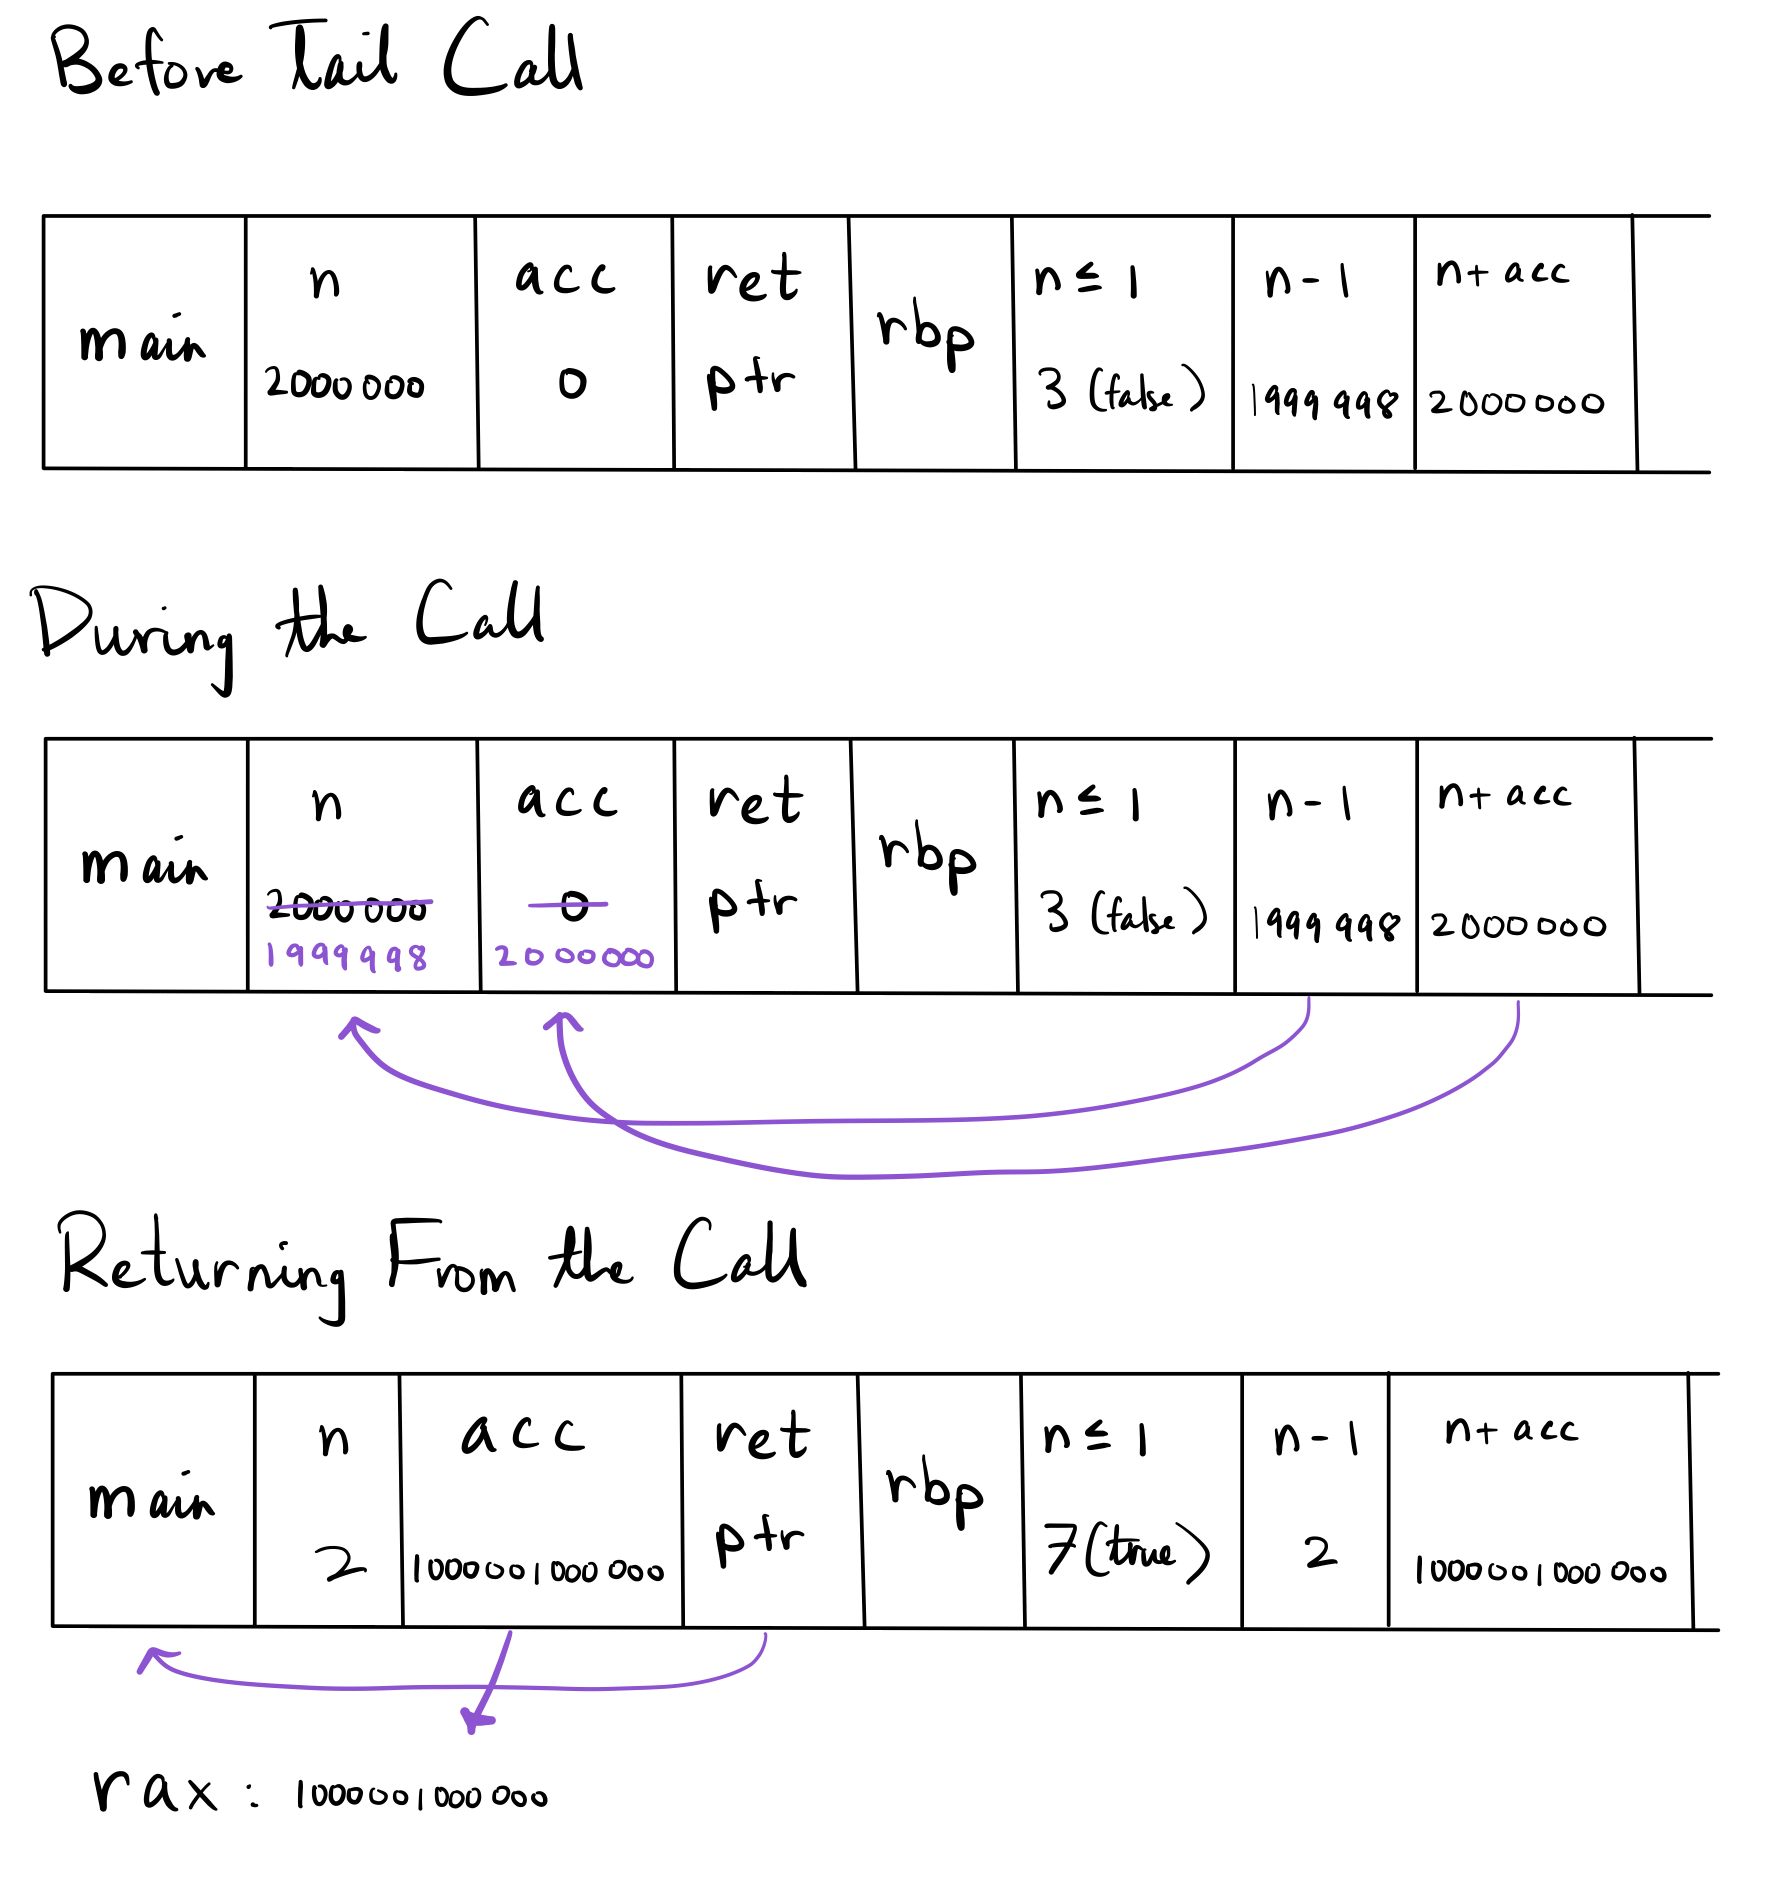
\includegraphics[scale=0.25]{stack.png}
\end{center}

\section{Tail Call Tests}
\subsection{Test 1}
Our first test is the following
\begin{verbatim}
(fun (sum n acc)
    (if (< n 1)
        acc
        (sum (sub1 n) (+ n acc))
    )
)

(sum 1000000 0)\end{verbatim}

This program recursively computes the sum of the first $n$ (or 1000000 in our case) numbers, 
using an accumulator and recursive tail calls. \newline

When compiled and run, it outputs \verb|500000500000| as desired.

\subsection{Test 2}
Our second test is the following
\begin{verbatim}
(fun (even n)
    (if (= n 0)
        true
        (odd (sub1 n))
    )
)

(fun (odd n)
    (if (= n 1)
        true
        (even (sub1 n))
    )
)

(even 1000000)\end{verbatim}
This program determines if the inputted integer ($1000000$ in our case) is even or not. The even function uses
the odd function as a helper function and they call each other mutual recursively to arrive at the correct
answer. \newline

When compiled and run, this program outputs \verb|even| as desired.

\subsection{Test 3}
Our third test is the following
\begin{verbatim}
(fun (sum-of-squares acc n)
    (if (= n 1)
        (+ acc 1)
        (sum-of-squares (+ acc (* n n)) (sub1 n))
    )
)
(sum-of-squares 0 1000000)\end{verbatim}
This program recursively computes the sum of the squares of the first $n$ (or 1000000 in our 
case) positive integers, using an accumulator and recursive tail calls. In other words, it computes
$\sum_{k=1}^n k^2$ for any inputted $n\geq1$. \newline

When compiled and run, it outputs \verb|333333833333500000| as desired.
\section{Resources Used}
I used multiple different websites as references for calling conventions, tail calls, and x86\_86 assembly. I've
listed them below.
\begin{itemize}
    \item\url{https://course.ccs.neu.edu/cs4410sp20/lec_tail-calls_stack_notes.html} 
    \item \url{https://eklitzke.org/how-tail-call-optimization-works} 
    \item \url{https://courses.cs.cornell.edu/cs3110/2021sp/textbook/data/tail_recursion.html}
    \item \url{https://aaronbloomfield.github.io/pdr/book/x86-64bit-ccc-chapter.pdf}
\end{itemize}
\end{document}
